\documentclass{article}

\usepackage[english]{babel}
\usepackage[letterpaper,top=2cm,bottom=2cm,left=3cm,right=3cm,marginparwidth=1.75cm]{geometry}
\usepackage{amsmath}
\usepackage{graphicx}
\usepackage{booktabs}
\usepackage{array}
\usepackage{setspace}
\usepackage{enumitem}
\usepackage{caption}
\usepackage[colorlinks=true, allcolors=blue]{hyperref}

\graphicspath{{assets/}}
\newcolumntype{L}[1]{>{\raggedright\arraybackslash}p{#1}}

\setstretch{1.02}
\setlength{\parindent}{0pt}
\setlength{\parskip}{0.35em}
\captionsetup{font=small}

\title{LLM efficiency in analysis of animal behavior datasets}
\author{Ahren Berlanger, Ricardo Calvo Mendez, Samuel Senneka}

\begin{document}
\maketitle

\begin{abstract}
This study used design-of-experiments methods to evaluate the efficiency and structural reliability of large language models (LLMs) when asked to analyze a mouse navigation dataset. The source file contained 78{,}687 observations; 76{,}655 remained after filtering to the five required stimulation paradigms: Combined, ICMS Only, Dim Visual Only, Bright Visual Only, and Sham. Each model received only five performance variables: Time-to-Target, Success, Path Efficiency, Average Speed, and angular dispersion (AD). The experiment was a completely randomized full factorial with four treatment factors: model (DeepSeek-V3.1, Kimi-K2.5, Qwen3.5-9B), temperature (0, 0.25, 0.5, 0.75, 1.0), prompt template (basic, ANOVA, predictive), and data view (summary only, stimulus summary, stimulus plus mouse summary). Three replications per treatment combination yielded 405 runs.

The completed experiment consumed 1{,}389{,}891 total tokens and produced valid JSON in 377 runs (93.1\%) under a fixed 1{,}800-token output cap. Data view dominated token usage ($F=6311.74$, $p<2.2\times10^{-227}$, $\eta^2=0.846$), with model and the model-by-data-view interaction as secondary contributors. Runtime was driven primarily by model ($F=58.47$, $p<8.1\times10^{-22}$, $\eta^2=0.212$). DeepSeek-V3.1 was fastest on average (17.9 s), Kimi-K2.5 slowest (38.3 s), and Qwen3.5-9B intermediate (28.1 s). Qwen3.5-9B achieved 100\% valid JSON, Kimi-K2.5 97.0\%, and DeepSeek-V3.1 82.2\%, with all invalid outputs attributable to length-capped generations. The observed Together AI spend was approximately \$1.11, so three replications were economically feasible. Overall, model choice and data packaging had much larger practical effects than temperature.
\end{abstract}

\section{Introduction}

Large language models are increasingly used as lightweight analysis assistants for scientific data, but their practical behavior depends on model family, prompt specificity, and the amount of context supplied at inference time. This makes LLM evaluation a natural design-of-experiments (DOE) problem: analysts can manipulate several controllable factors, randomize runs, replicate treatment combinations, and measure cost, latency, and output reliability using standard DOE principles \cite{montgomery,boxhunter}.

The motivating scientific context for this project was a mouse navigation dataset shared within the course team. The biological question concerns performance under five stimulation paradigms: Combined, ICMS Only, Dim Visual Only, Bright Visual Only, and Sham. Rather than re-running the biological experiment itself, the present study treats the \emph{LLM analysis pipeline} as the experimental system. The operational question was:

\begin{quote}
\textbf{How do model choice, temperature, prompt specificity, and data-view complexity affect the computational and structural performance of LLM-generated statistical analyses?}
\end{quote}

That question matters for practical reasons. A model that appears analytically capable but is slow, expensive, or structurally unreliable may be a poor fit for routine coursework or exploratory scientific use. The goal of this report is therefore not to certify the truthfulness of each model's scientific interpretation, but to quantify how controllable design choices influence efficiency, robustness, and reproducibility.

\section{Methods}

\subsection{Experimental Units, Treatments, and Blocking}

The experimental unit was one completed LLM analysis run. Each run combined one model, one temperature level, one prompt template, and one data view. The input data were stored in \texttt{data.csv}. The original file contained 78{,}687 rows; 76{,}655 remained after filtering to the five required stimulation paradigms. The retained analytic columns were \texttt{Mouse}, \texttt{Stim Paradigm}, \texttt{Time-to-Target}, \texttt{Success}, \texttt{Path Efficiency}, \texttt{Average Speed}, and \texttt{AD}. No missing values remained in the filtered dataset.

Table~\ref{tab:source-summary} summarizes the source-data pattern seen by the models. Combined and Bright Visual Only had the highest mean success and shortest average time-to-target, whereas Sham was substantially worse on both dimensions. Figure~\ref{fig:source-context} gives the same story graphically for the two most interpretable outcomes. These visible differences ensured that the models were given a meaningful statistical pattern to describe.

\begin{table}[tbp]
\centering
\caption{Filtered source-data summary by stimulation paradigm}
\label{tab:source-summary}
\small
\begin{tabular}{lrrrrrr}
\toprule
Stim paradigm & $n$ & Success & Time-to-target & Path eff. & Avg. speed & AD \\
\midrule
Bright Visual Only & 3{,}323 & 0.785 & 2.614 & 0.504 & 12.679 & 0.387 \\
Combined & 48{,}846 & 0.780 & 2.562 & 0.502 & 12.833 & 0.399 \\
Dim Visual Only & 9{,}603 & 0.673 & 3.140 & 0.434 & 11.968 & 0.336 \\
ICMS Only & 11{,}378 & 0.685 & 3.053 & 0.432 & 12.039 & 0.354 \\
Sham & 3{,}505 & 0.273 & 4.682 & 0.308 & 10.737 & 0.236 \\
\bottomrule
\end{tabular}
\end{table}

\begin{figure}[tbp]
\centering
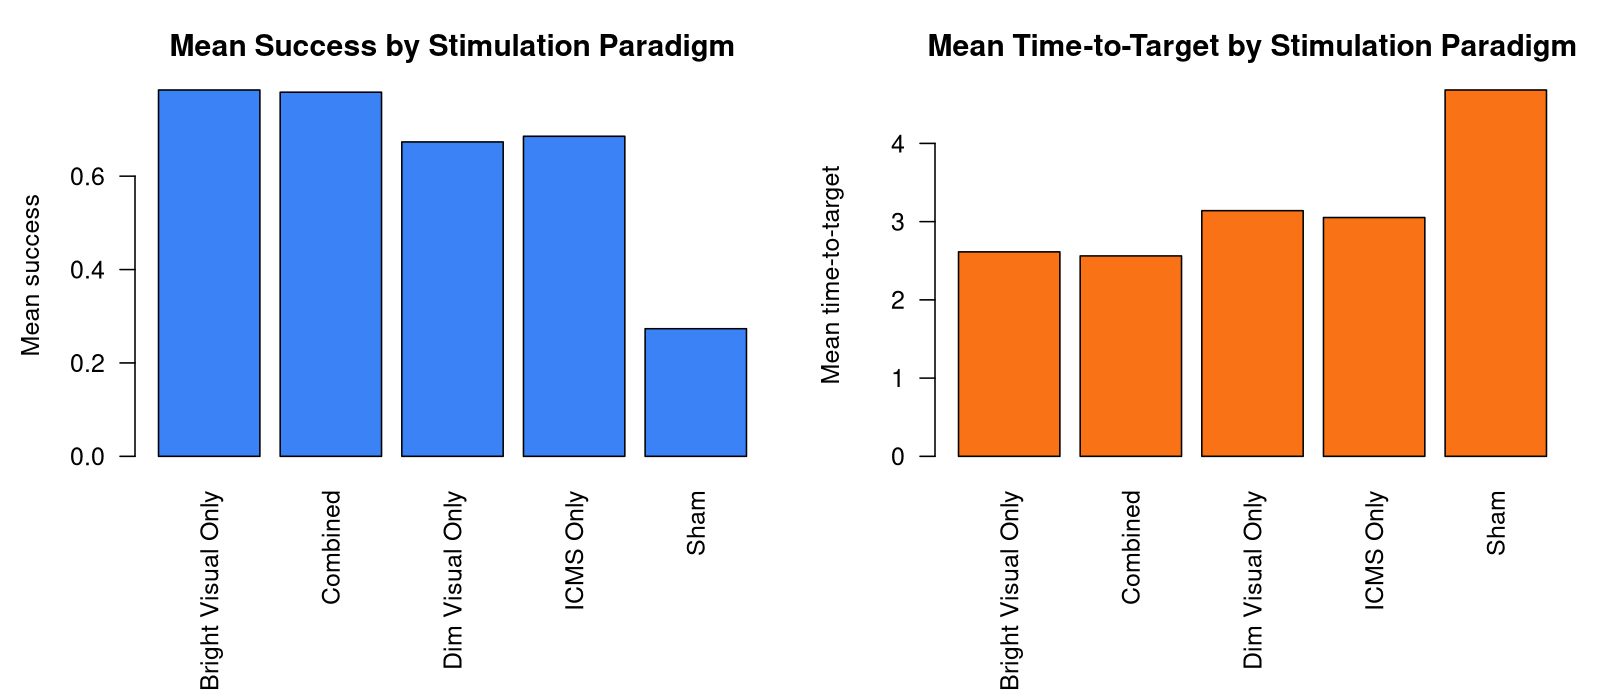
\includegraphics[width=\textwidth]{figure_source_data_context.png}
\caption{Source-data context supplied to the LLMs. Sham is visibly worst on both mean success and mean time-to-target.}
\label{fig:source-context}
\end{figure}

The treatment factors are listed in Table~\ref{tab:design-factors}. No formal blocking factor was introduced. All runs were executed through the same Together AI serverless interface under the same Python pipeline, so nuisance variation was handled through randomization and replication rather than explicit blocks. In effect, backend variability and stochastic generation noise were absorbed into the run-level error term.

\begin{table}[tbp]
\centering
\caption{Design factors and levels}
\label{tab:design-factors}
\small
\begin{tabular}{L{1.7cm}L{5.6cm}L{5.2cm}}
\toprule
Factor & Levels & Notes \\
\midrule
Model & 3: DeepSeek-V3.1, Kimi-K2.5, Qwen3.5-9B & Together AI serverless models with reasoning disabled \\
Temperature & 5: 0.00, 0.25, 0.50, 0.75, 1.00 & Treated as a categorical factor \\
Prompt template & 3: basic, ANOVA, predictive & Increasing inferential specificity \\
Data view & 3: \texttt{summary\_only}, \texttt{stim\_summary}, \texttt{stim\_and\_mouse\_summary} & Controls how much context is exposed \\
Replication & 3 repeated runs per treatment combination & $3\times5\times3\times3\times3=405$ runs \\
\bottomrule
\end{tabular}
\end{table}

\subsection{Randomization and replication plan}

The experiment was a balanced, completely randomized full factorial design with 135 unique treatment combinations and 3 replications per treatment combination, for a planned total of 405 runs. Run order was randomized using seed \texttt{51400}. Replication served two purposes. First, it captured stochastic response variation from the models. Second, because the models were accessed through a cloud service, replication also captured transient service variability such as latency fluctuations and occasional API failures.

The initial live sweep produced 7 API failures, including timeouts and a transient 503 response. Those failed runs were rerun so that the final dataset contained all 405 planned observations. This is important for the factorial analysis because it preserves balance across treatment combinations and simplifies interpretation of main effects and interactions.

\subsection{Execution and data collection}

The execution pipeline was implemented in Python 3.14.4 \cite{python} and used Together AI as the live inference backend \cite{togetherchat,togetherjson,togethermodels}. The evaluated model families were DeepSeek-V3.1, Kimi-K2.5, and Qwen3.5-9B. The project codebase contained 10 Python source modules totaling 1{,}472 source lines and 193 test lines. Report-side summaries and figures were generated in R \cite{rcore}. Pinned runtime dependencies were \texttt{python-dotenv==1.2.2} and \texttt{together==2.12.0}.

Each run recorded wall-clock runtime, input tokens, output tokens, total tokens, stop reason, JSON validity, and schema completeness. The output budget was fixed at 1{,}800 generated tokens per run. Twenty-eight completed responses hit that cap and were structurally invalid because truncation interrupted the requested JSON format.

\section{Statistical analysis}

\subsection{Model specifications}

Three outcomes were analyzed:
\begin{enumerate}[leftmargin=1.7em]
    \item \texttt{total\_token\_count} as a direct proxy for usage cost,
    \item \texttt{wall\_clock\_seconds} as a latency measure, and
    \item \texttt{response\_json\_valid} as a structural reliability indicator.
\end{enumerate}

For the continuous outcomes, the primary full-factorial ANOVA models were
\[
\texttt{total\_token\_count} \sim \texttt{model} * \texttt{temperature} * \texttt{prompt} * \texttt{data\_view}
\]
and
\[
\log(\texttt{wall\_clock\_seconds}) \sim \texttt{model} * \texttt{temperature} * \texttt{prompt} * \texttt{data\_view}.
\]

Runtime was log-transformed because raw runtimes were right-skewed and bounded below by zero. For structured-output validity, the primary model was an additive logistic regression,
\[
\operatorname{logit}\{P(\texttt{valid JSON})\} \sim \texttt{model} + \texttt{temperature} + \texttt{prompt} + \texttt{data\_view},
\]
because perfect validity for Qwen3.5-9B creates separation problems in richer binary-outcome models.

The ANOVA assumptions were the usual ones: independent run-level errors, mean-zero residuals, approximately constant variance for the transformed continuous outcomes, and correct functional form for the logistic model. Because the design was fully balanced and the strongest effects were very large, moderate deviations from homoscedasticity were not expected to overturn the main practical conclusions.

\subsection{Planned contrasts and hypotheses}

Primary hypotheses were all two-sided and evaluated at $\alpha = 0.05$. The central hypotheses were:
\begin{enumerate}[leftmargin=1.7em]
    \item model family affects token usage, runtime, and JSON validity;
    \item temperature affects one or more outcomes;
    \item prompt specificity affects one or more outcomes; and
    \item data-view complexity affects one or more outcomes, possibly through interactions with model.
\end{enumerate}

After the omnibus ANOVA tests, pairwise follow-up comparisons were planned using Tukey HSD for the continuous outcomes most relevant to interpretation: model differences in log-runtime and data-view differences in total tokens. The report emphasizes effect sizes and practical meaning rather than significance alone, because the purpose of the study is to guide workflow design rather than only to reject null hypotheses.

\subsection{Diagnostics}

Residual-versus-fitted and Q--Q diagnostics were inspected during the longer analysis workflow. The main diagnostic result was that the log transform improved runtime residual behavior substantially. Token residuals still showed mild heteroskedasticity at the largest fitted values, which is unsurprising because the richest data view creates a visibly different scale of responses. However, the overwhelming dominance of data view and the large model effects were stable enough that these modest departures were not treated as a threat to the main interpretation.

\begin{figure}[tbp]
\centering
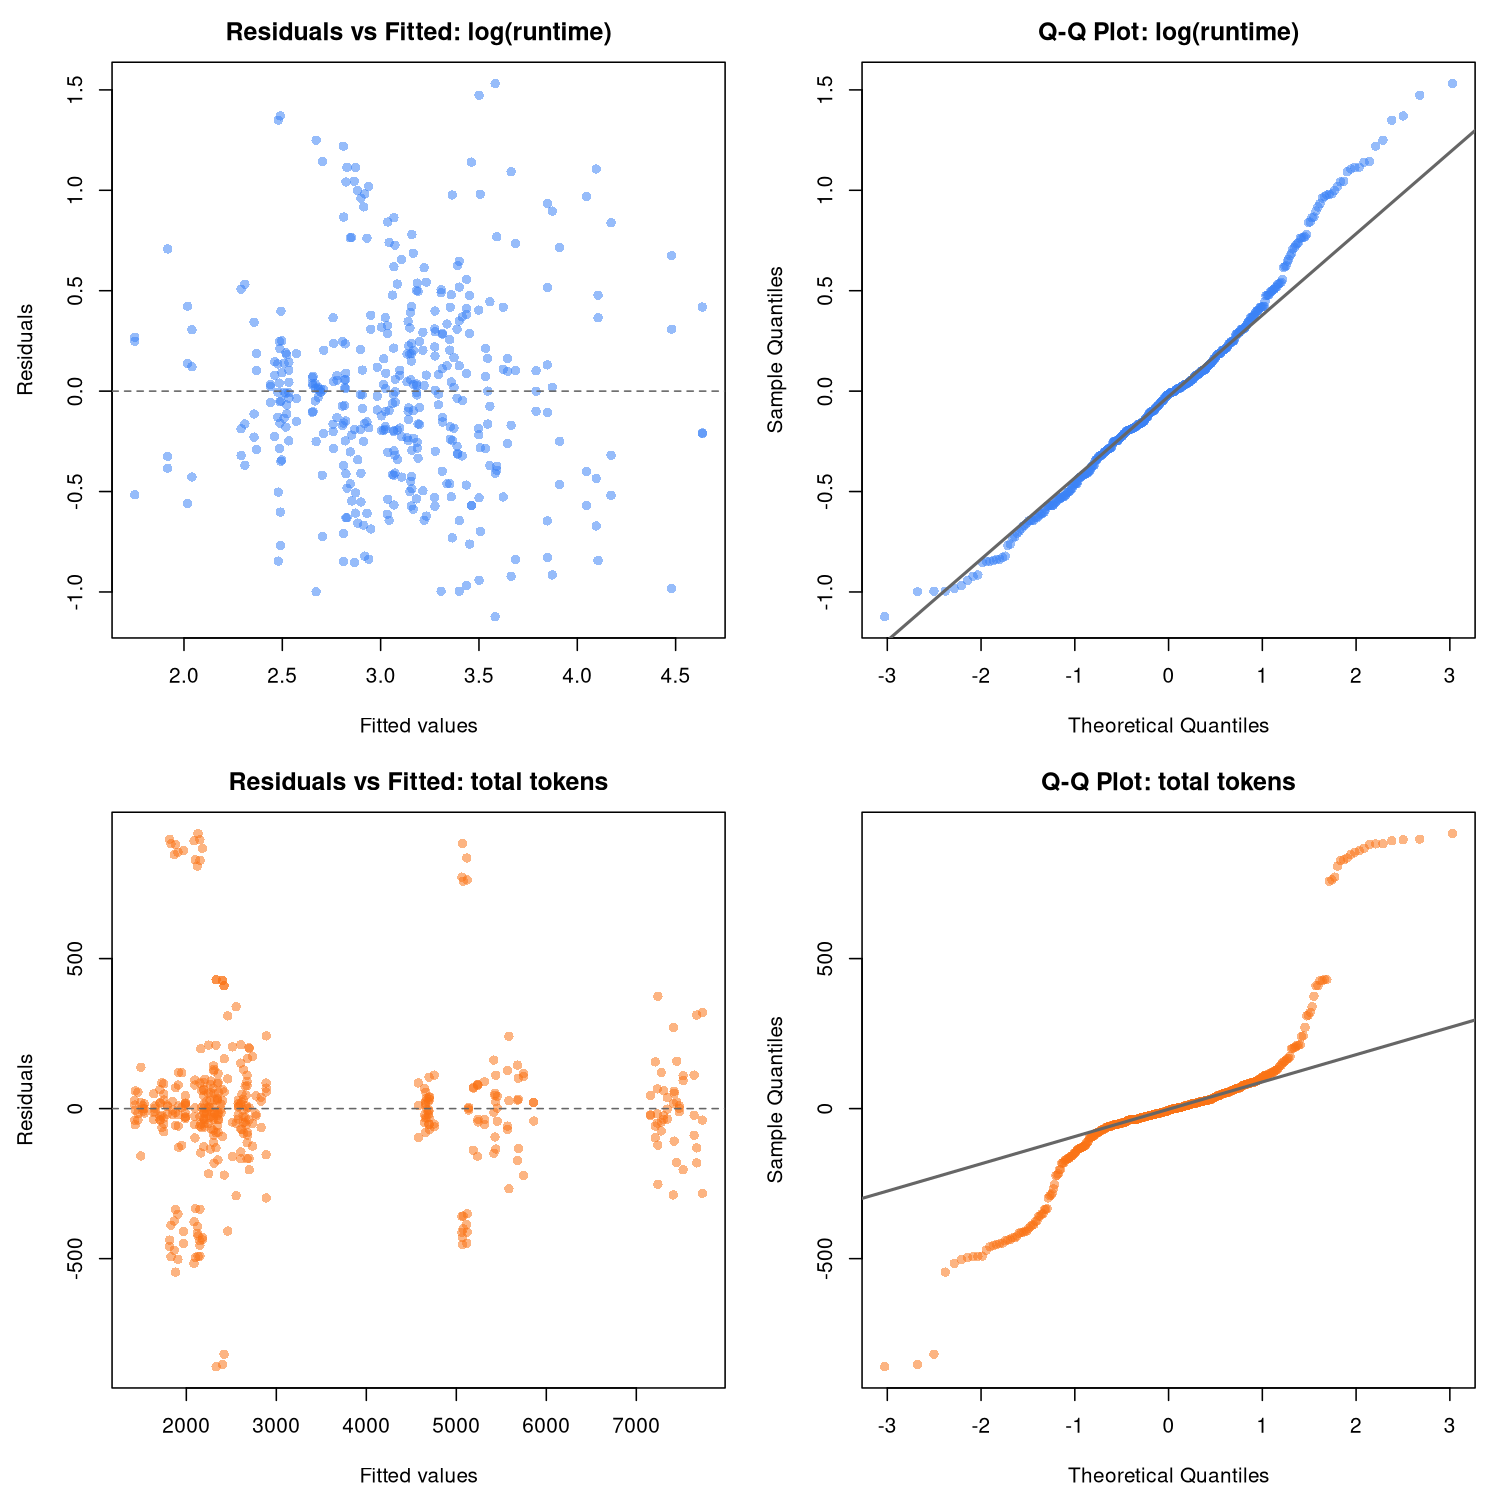
\includegraphics[width=\textwidth]{figure_diagnostics.png}
\caption{Residual and Q--Q diagnostics for the log-runtime and total-token ANOVA models. The log transform improved runtime behavior, while token residuals still showed mild scale-related departures at the largest fitted values.}
\label{fig:diagnostics}
\end{figure}

\subsection{Sensitivity / Robustness Analysis}

Several checks were used to confirm that the main conclusions were not artifacts of a single modeling choice. First, runtime was analyzed on the log scale because raw runtime was right-skewed; the ranking of models did not change after this transformation. Second, the token model was inspected for heteroskedasticity, and although the richest data view produced somewhat larger residual spread, the dominant data-view effect was so large that the substantive ranking of factors was unchanged. Third, I recomputed the descriptive runtime and token summaries on the subset of runs with \texttt{done\_reason = "stop"} only. The ordering remained the same: DeepSeek-V3.1 was fastest, Kimi-K2.5 was slowest, and Qwen3.5-9B was most token-intensive. Finally, malformed JSON outputs were treated conservatively as failures rather than silently dropped. This is important because all invalid outputs were caused by the fixed 1{,}800-token cap, so the structural-validity conclusions should be interpreted explicitly as \emph{validity under a capped-output workflow}. None of these checks changed the qualitative conclusions about the relative importance of model choice and data-view complexity.

\section{Results}

\subsection{Descriptive statistics in summary tables}

The final dataset contained all 405 planned runs. Table~\ref{tab:project-summary} summarizes the overall experiment. The run consumed 953{,}145 input tokens, 436{,}746 output tokens, and 1{,}389{,}891 tokens in total. Mean runtime was 28.10 seconds per run. The observed Together AI spend was approximately \$1.11, which implies a mean cost of roughly \$0.00274 per run. This low cost strongly justified the decision to use three replications per treatment combination.

\begin{table}[tbp]
\centering
\caption{Overall experiment summary}
\label{tab:project-summary}
\small
\begin{tabular}{lr}
\toprule
Metric & Value \\
\midrule
Completed runs & 405 \\
Treatment combinations & 135 \\
Replications per treatment & 3 \\
Valid JSON responses & 377 \\
JSON validity rate & 93.1\% \\
Length-capped responses & 28 \\
Total input tokens & 953{,}145 \\
Total output tokens & 436{,}746 \\
Total tokens & 1{,}389{,}891 \\
Mean wall-clock seconds per run & 28.10 \\
Reported Together cost (USD) & \$1.11 \\
\bottomrule
\end{tabular}
\end{table}

Table~\ref{tab:model-summary} shows the basic model-level tradeoff. DeepSeek-V3.1 was fastest and least token-intensive on average, but also the least reliable structurally under the fixed 1{,}800-token cap. Kimi-K2.5 was the slowest model yet highly stable. Qwen3.5-9B consumed the most tokens, but it was the only model with perfect JSON validity across the balanced final dataset.

\begin{table}[tbp]
\centering
\caption{Model-level descriptive summary ($n=135$ runs per model)}
\label{tab:model-summary}
\small
\resizebox{\textwidth}{!}{%
\begin{tabular}{lrrrr}
\toprule
Model & Runtime, s (approx.\ 95\% CI) & Total tokens (95\% CI) & Valid JSON, \% (95\% CI) & Length-cap, \% \\
\midrule
DeepSeek-V3.1 & 17.9 [16.2, 19.8] & 2{,}847 [2{,}794, 2{,}900] & 82.2 [74.9, 87.8] & 17.8 \\
Kimi-K2.5 & 38.3 [34.7, 42.3] & 3{,}375 [3{,}322, 3{,}428] & 97.0 [92.6, 98.8] & 3.0 \\
Qwen3.5-9B & 28.1 [25.4, 31.0] & 4{,}073 [4{,}020, 4{,}126] & 100.0 [97.2, 100.0] & 0.0 \\
\bottomrule
\end{tabular}
}
\caption*{\footnotesize Runtime intervals are approximate 95\% intervals obtained by back-transforming the pooled log-runtime error term. Token intervals use the common pooled ANOVA error term. Validity intervals are Wilson 95\% binomial intervals.}
\end{table}

\subsection{ANOVA or model summary table}

Table~\ref{tab:anova-selected} reports the most relevant factorial effects. For total token usage, data view was by far the dominant factor ($F=6311.74$, $p<2.2\times10^{-227}$, $\eta^2=0.846$), followed by model ($F=522.62$, $p<1.5\times10^{-93}$) and the model-by-data-view interaction ($F=200.28$, $p<1.7\times10^{-79}$). Temperature had no meaningful main effect on total tokens ($F=0.85$, $p=0.493$). For runtime, model was again the dominant factor ($F=58.47$, $p<8.1\times10^{-22}$, $\eta^2=0.212$), with a smaller but still statistically significant prompt effect ($F=7.06$, $p=0.0010$).

\begin{table}[tbp]
\centering
\caption{Selected ANOVA results for the primary continuous outcomes}
\label{tab:anova-selected}
\small
\begin{tabular}{L{2.1cm}L{4.8cm}rrr}
\toprule
Outcome & Term & $F$ & $p$-value & $\eta^2$ \\
\midrule
Total tokens & Data view & 6311.74 & $<2.2\times10^{-227}$ & 0.846 \\
Total tokens & Model & 522.62 & $<1.5\times10^{-93}$ & 0.070 \\
Total tokens & Model $\times$ Data view & 200.28 & $<1.7\times10^{-79}$ & 0.054 \\
Log runtime & Model & 58.47 & $<8.1\times10^{-22}$ & 0.212 \\
Log runtime & Prompt & 7.06 & 0.0010 & 0.026 \\
Log runtime & Temperature $\times$ Prompt & 2.23 & 0.0257 & 0.032 \\
\bottomrule
\end{tabular}
\end{table}

\subsection{Plots showing estimated effects, confidence intervals, and interactions}

Figure~\ref{fig:runtime} shows the model-level runtime ordering. Kimi-K2.5 was the slowest model, Qwen3.5-9B intermediate, and DeepSeek-V3.1 fastest. Tukey contrasts on log-runtime indicated that all three pairwise differences were statistically significant, with Kimi-K2.5 slower than both alternatives and Qwen3.5-9B slower than DeepSeek-V3.1.

\begin{figure}[tbp]
\centering
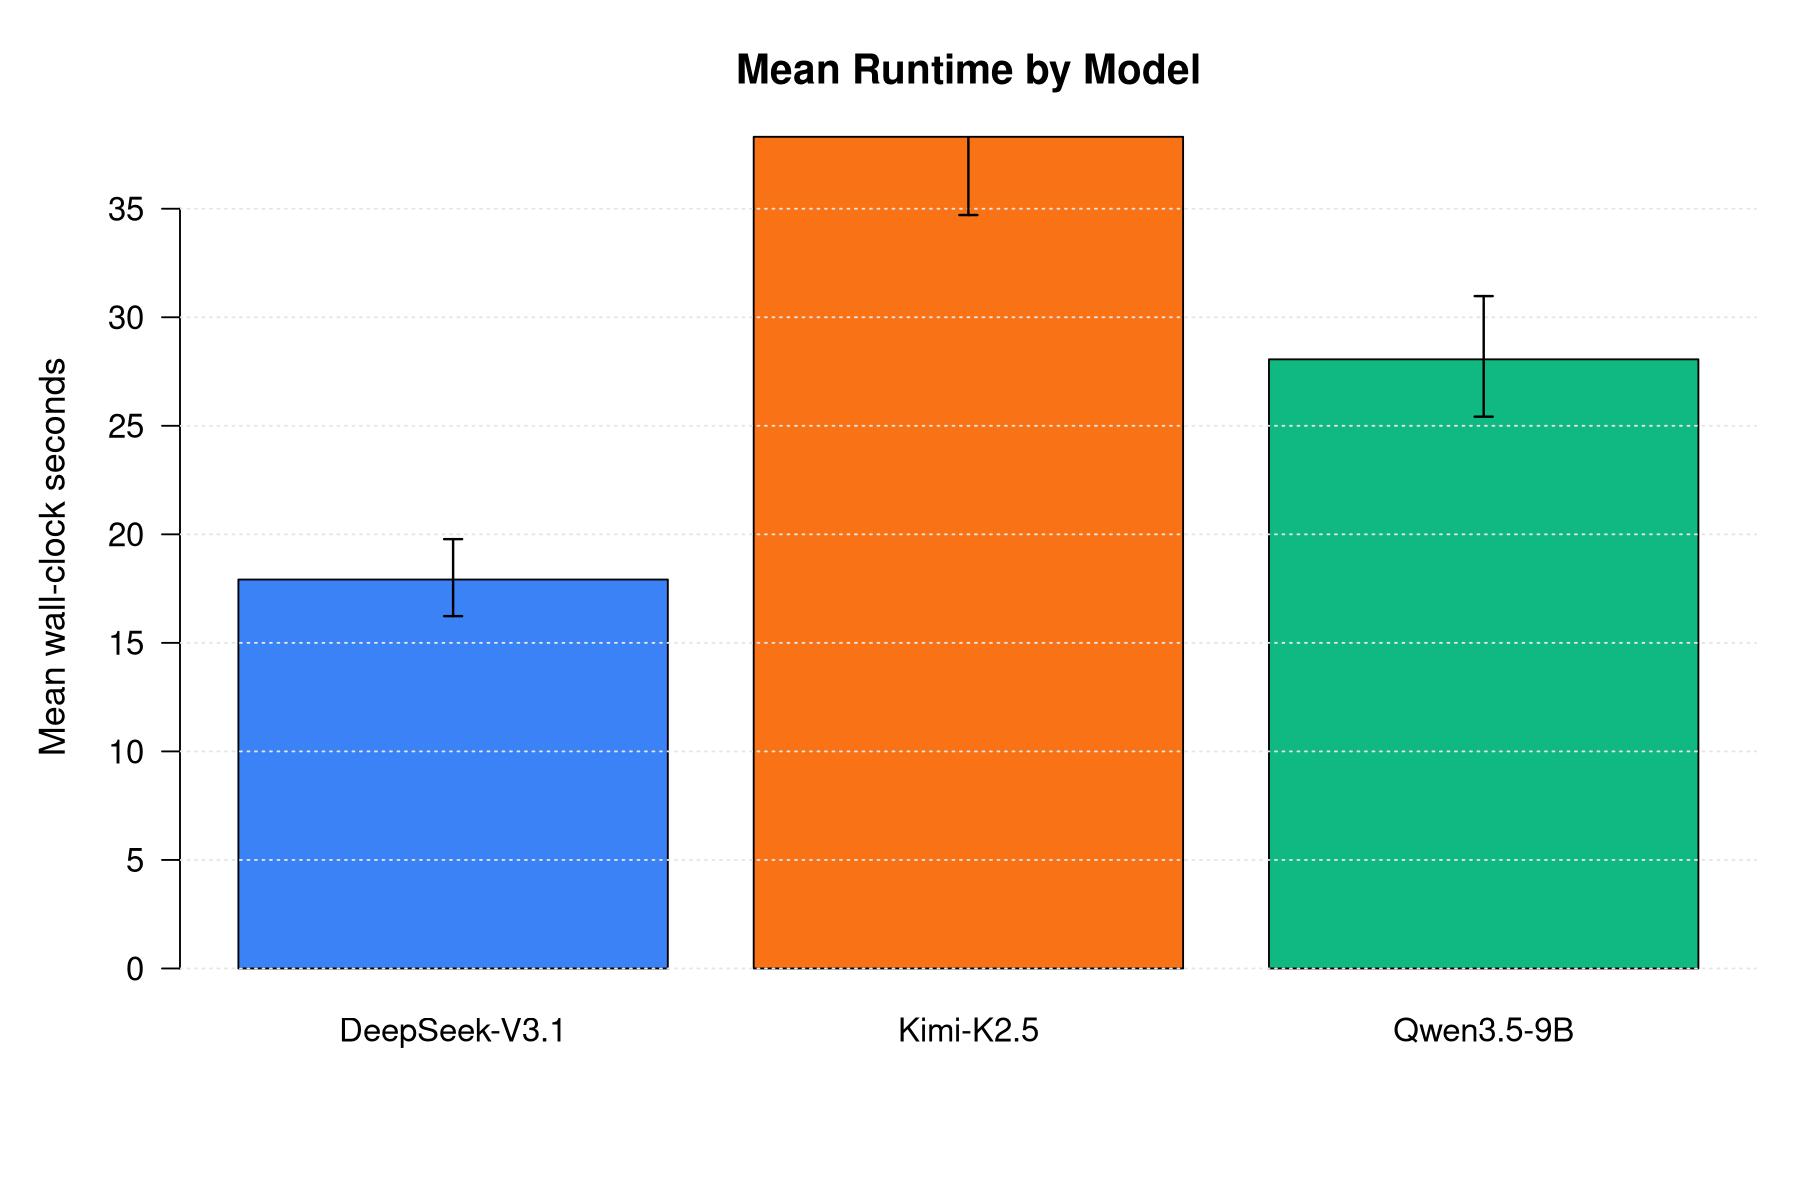
\includegraphics[width=0.82\textwidth]{figure_model_runtime_mean_clean.png}
\caption{Mean wall-clock runtime by model with approximate 95\% intervals derived from the pooled log-runtime error term. Model choice was the dominant runtime factor.}
\label{fig:runtime}
\end{figure}

Figure~\ref{fig:token-interaction} shows the most important interaction in the study. The richest data view sharply increased token usage for all models, but most dramatically for Qwen3.5-9B. Mean total tokens under that richest view were approximately 4{,}813 for DeepSeek-V3.1, 5{,}465 for Kimi-K2.5, and 7{,}406 for Qwen3.5-9B.

\begin{figure}[tbp]
\centering
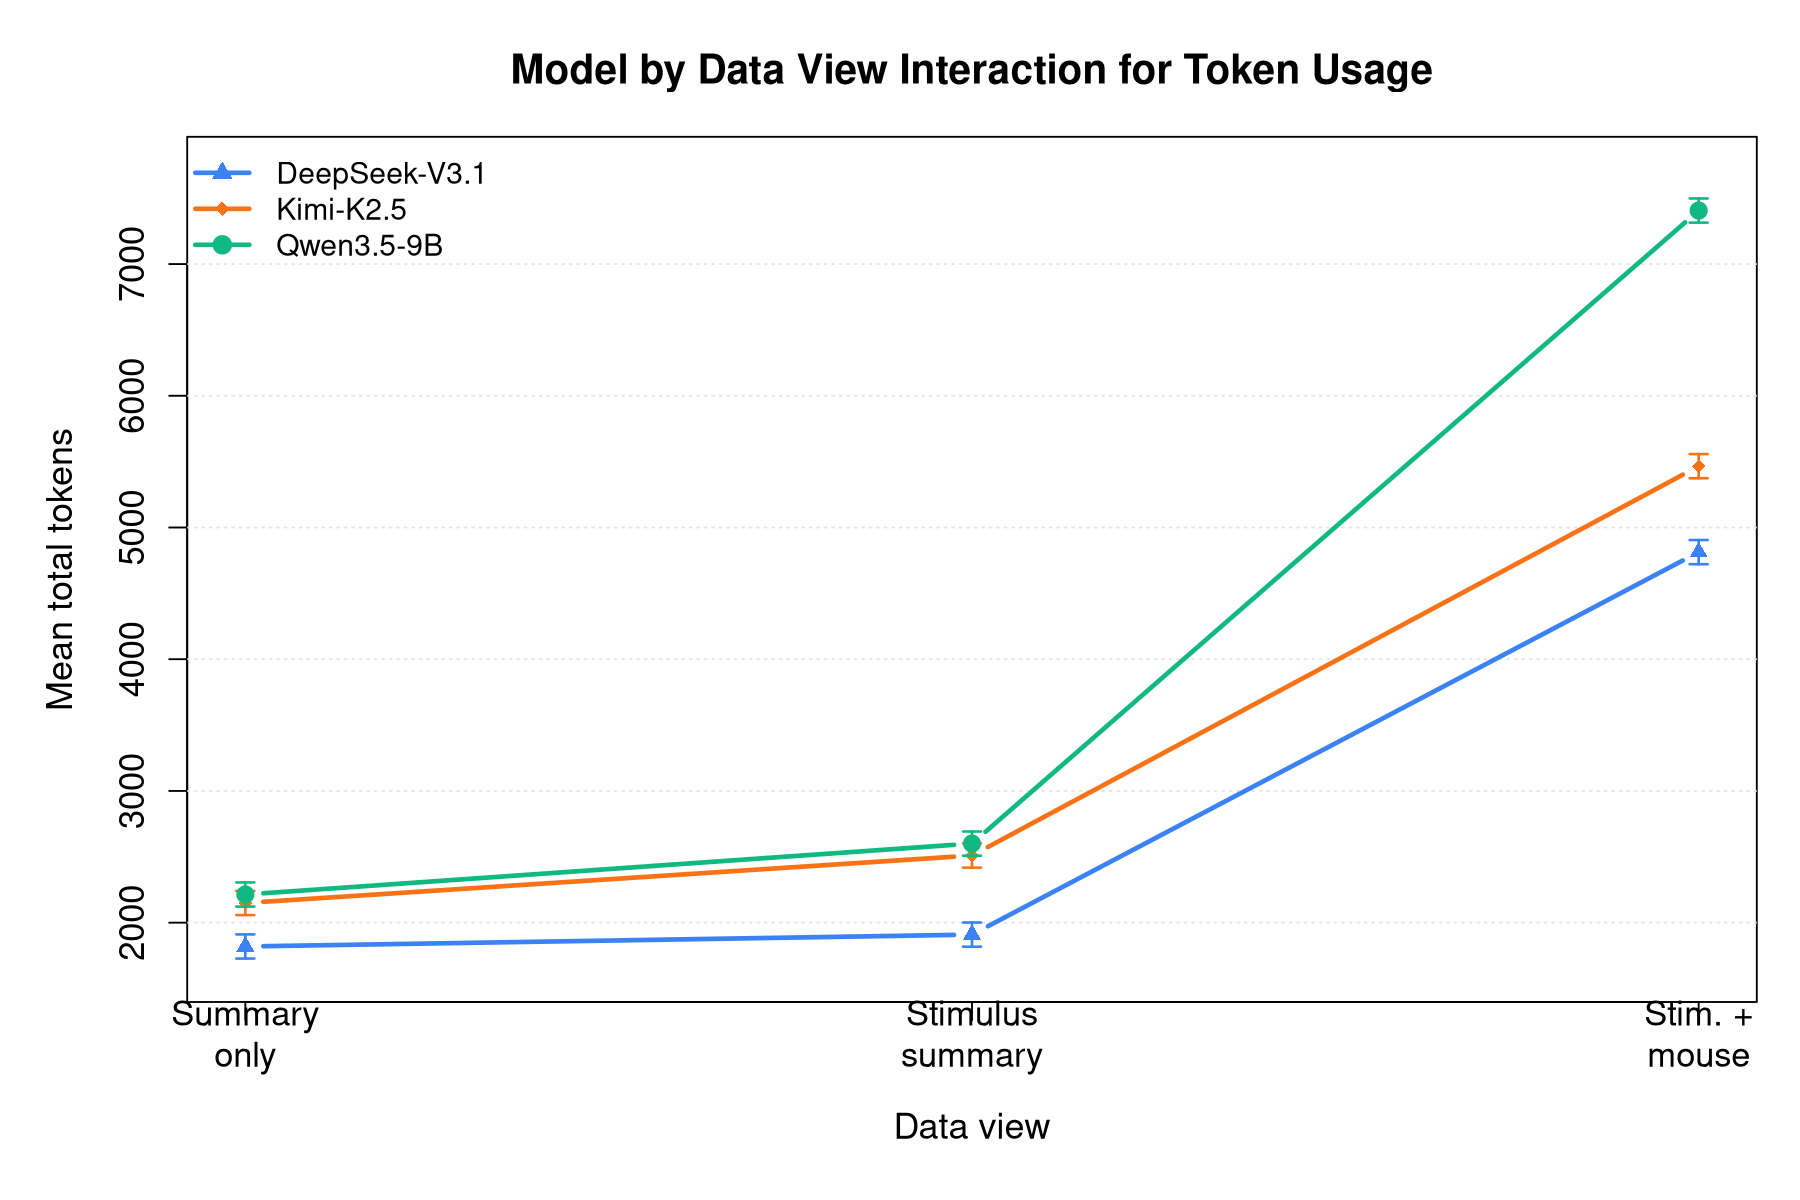
\includegraphics[width=\textwidth]{figure_model_data_view_tokens_clean.png}
\caption{Model-by-data-view interaction for token usage. Error bars show common 95\% intervals from the pooled ANOVA error term. Context packaging was the dominant cost lever in the experiment.}
\label{fig:token-interaction}
\end{figure}

Figure~\ref{fig:validity} summarizes structural reliability. Qwen3.5-9B was uniformly valid across prompt types, Kimi-K2.5 remained near-perfect, and DeepSeek-V3.1 showed noticeably lower validity. All invalid outputs in the completed dataset corresponded to length-capped generations, so the reliability problem was directly tied to truncation rather than arbitrary schema drift.

\begin{figure}[tbp]
\centering
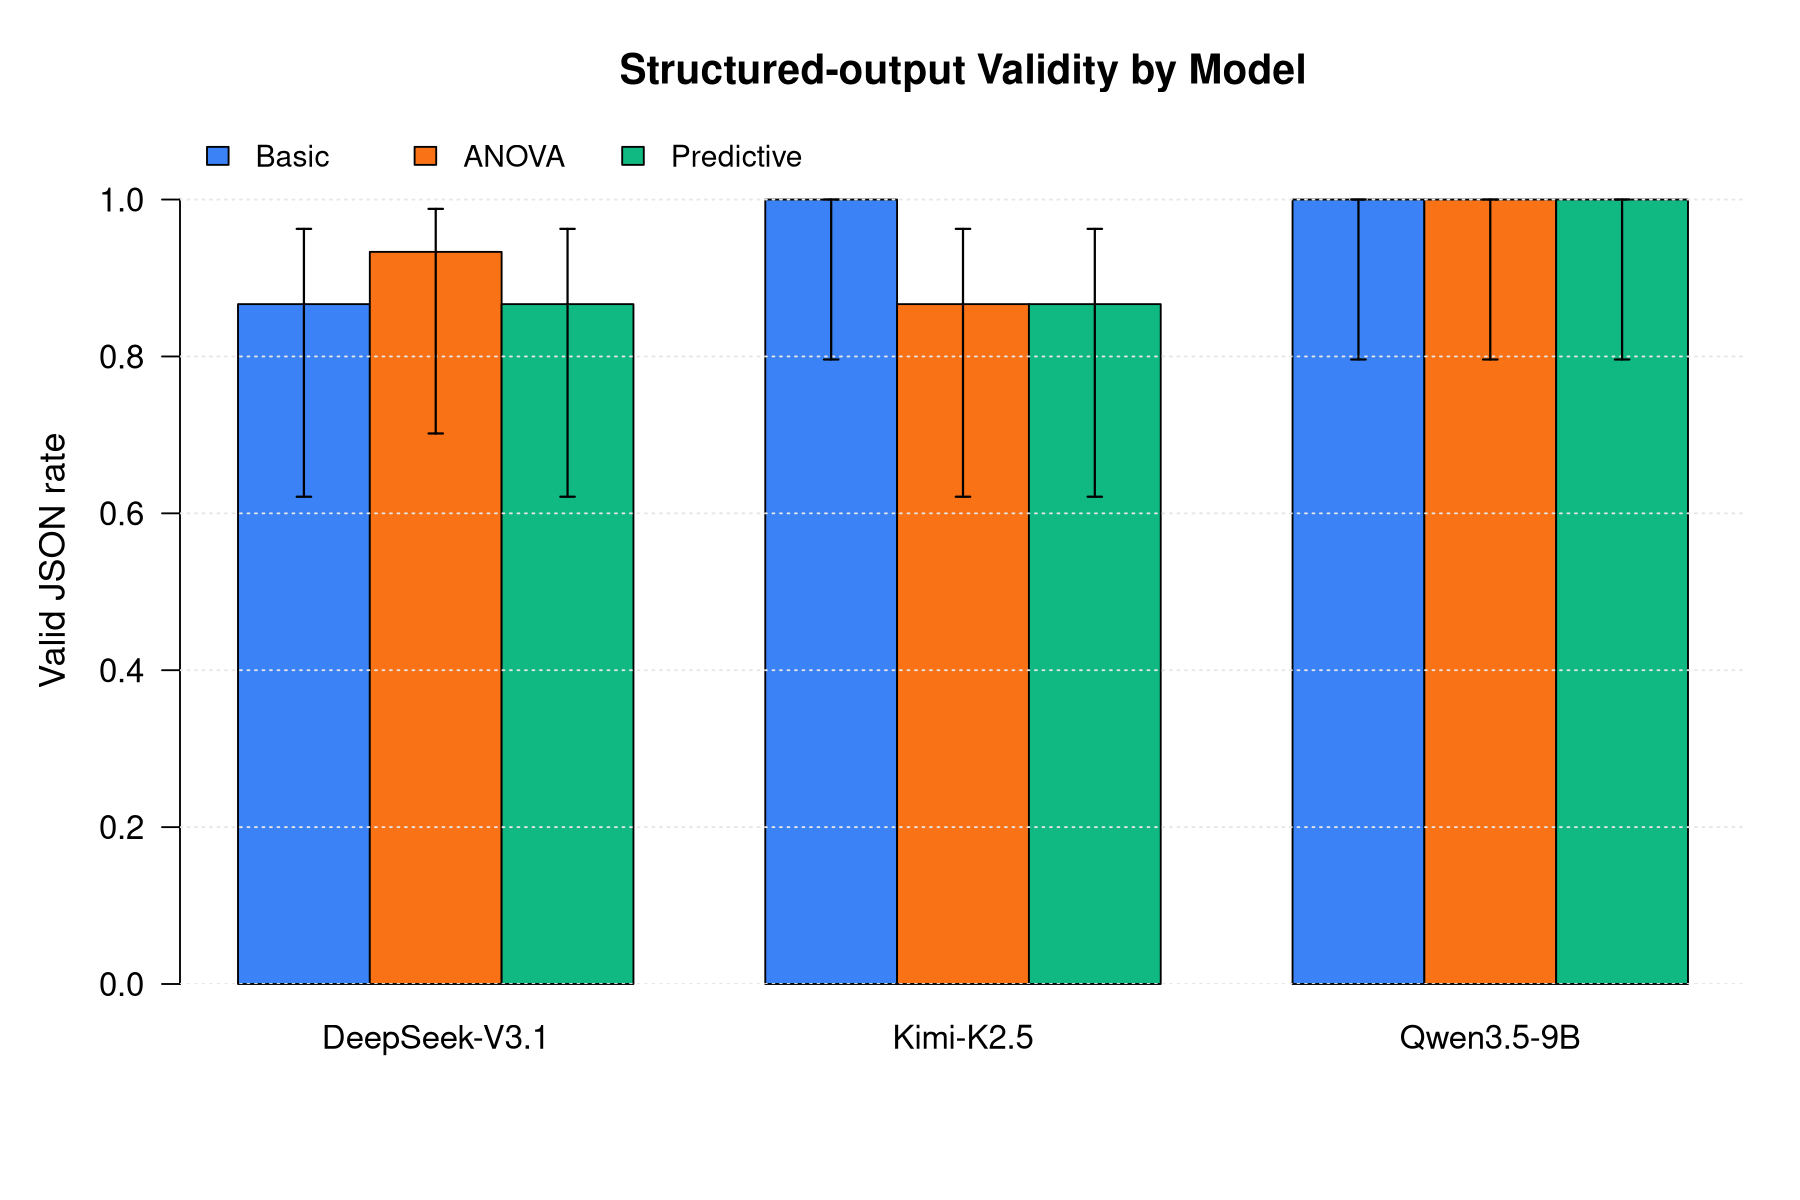
\includegraphics[width=0.95\textwidth]{figure_validity_by_model_prompt_clean.png}
\caption{Structured-output validity by model and prompt within the richest data view, under the fixed 1{,}800-token output cap. Error bars are Wilson 95\% intervals with $n=15$ runs per bar. Reliability was primarily a model effect, not a temperature effect.}
\label{fig:validity}
\end{figure}

\subsection{Structured-output validity}

Structured-output validity was defined narrowly: the response had to be valid JSON that matched the required top-level schema. Under that criterion, the overall validity rate was 93.1\%, but this should be interpreted specifically as validity under the fixed 1{,}800-token output cap.

The additive logistic model showed that model family was the only clearly important predictor of validity. Table~\ref{tab:validity-model} summarizes the inferential results. Temperature, prompt, and data view were not significant once model was included in the additive specification. Descriptively, the separation is also large: Table~\ref{tab:model-summary} shows that DeepSeek-V3.1 remained well below the other two models even after binomial uncertainty is reflected through 95\% confidence intervals.

\begin{table}[tbp]
\centering
\caption{Additive logistic model summary for valid JSON}
\label{tab:validity-model}
\small
\begin{tabular}{lrr}
\toprule
Term & Test statistic & $p$-value \\
\midrule
Model & LR $\chi^2 = 41.80$ & $8.38\times10^{-10}$ \\
Temperature & --- & 0.625 \\
Prompt template & --- & 0.441 \\
Data view & --- & 0.441 \\
\bottomrule
\end{tabular}
\caption*{\footnotesize The additive form was used because Qwen3.5-9B achieved perfect validity, which creates separation problems in richer logistic models.}
\end{table}

\subsection{What do the effects mean practically?}

The practical interpretation is straightforward. First, \emph{data packaging is the dominant cost lever}. The shift from a summary-only input to the richest stimulus-plus-mouse summary increased token usage far more than any temperature change. Second, \emph{model choice creates a tradeoff among speed, reliability, and token cost}. DeepSeek-V3.1 was fast and relatively cheap but vulnerable to truncation; Kimi-K2.5 was slower but highly stable; Qwen3.5-9B was most reliable structurally but most token-expensive. Third, \emph{temperature mattered less than expected}. Across the main outcomes, temperature had little independent practical effect compared with model and data-view complexity.

\section{Discussion}

The key finding is that the computational behavior of LLM-based analysis pipelines is governed primarily by two design choices: which model is used and how much context is embedded in the prompt. This is a useful result for future coursework and small scientific projects because it shows that prompt-context engineering and model selection matter more than temperature sweeps when the objective is efficient, structured statistical output.

Several limitations should be acknowledged. The study measured computational efficiency and output structure, not substantive correctness of the models' scientific conclusions. A model can return valid JSON quickly while still making questionable inferential claims. In addition, the fixed output cap of 1{,}800 tokens created a real truncation mechanism, especially for DeepSeek-V3.1. That cap was methodologically useful because it standardized the runtime environment, but it also means that the JSON-validity findings should be interpreted as conditional on a capped-output workflow rather than as an absolute property of each model family.

From a DOE perspective, the design was efficient. A balanced 405-run experiment with three replications cost only about \$1.11, which is exceptionally cheap for a replicated cloud-based experiment. Replication was therefore easy to defend and helped absorb service-level variability that would otherwise have been confounded with treatment effects. The main practical challenge was not budget but the management of structured-output failures and reruns.

Future improvements are clear. The next iteration should add a rubric-based accuracy assessment, possibly combining instructor review with a rules-based checklist for whether the model identified the correct high-level pattern across stimulation paradigms. It would also be valuable to optimize context compression so that richer data views retain their statistical signal without creating such steep token penalties.

\section{Code and Data Availability}

All project materials are available at \href{https://github.com/rcalvom/STAT-51400-project}{https://github.com/rcalvom/STAT-51400-project} at commit \texttt{8b76d1e}. Python was used for experiment execution and Together AI interaction, while R was used to generate report-side summaries and figures. The final balanced results were obtained after rerunning the initial API failures so that all 405 planned runs were present in the completed dataset. Appendix~A lists the key repository paths and reproducibility materials.

\appendix
\section{Reproducibility Materials}

The repository contains the materials needed to reproduce the design and the report:
\begin{itemize}[leftmargin=1.7em]
    \item raw source dataset: \texttt{data.csv}
    \item derived prompt inputs and summaries: \texttt{artifacts/data/}
    \item experiment configuration: \texttt{configs/full\_factorial.json}
    \item randomization seed: \texttt{51400}
    \item generated design matrix path: \texttt{outputs/design\_matrix.csv}
    \item balanced run-level results: \texttt{outputs/results.csv}
    \item treatment-level summaries: \texttt{outputs/results\_summary.csv}
    \item Python execution pipeline: \texttt{src/llm\_doe/}
    \item submission-figure script: \texttt{analysis/generate\_submission\_figures.R}
    \item broader report-artifact script: \texttt{analysis/generate\_report\_artifacts.R}
    \item R session information: \texttt{report/tables/r\_session\_info.txt}
\end{itemize}

Within the repository, \texttt{data.csv} stores the raw source data. The deterministic prompt-facing summaries live in \texttt{artifacts/data/}, and the final run-level DOE outcomes live in \texttt{outputs/results.csv}.

\bibliographystyle{alpha}
\bibliography{sample}

\end{document}
